\chapter[Overlays, Groups, Girders, and Superpositions]
{Control Elements: Overlays, Groups, Girders, and Superpositions}
\label{c:control}
\index{element!control}
\index{element!lord}
\index{element!slave}
\index{tracking part}
It is possible to have elements controlling the attributes of other
elements. These \vn{lord} elements are meant, for example, to mimic
the effect of changing a knob in the control room. For this purpose
the lattice is split into two sections: The first section is the list
of elements that \bmad uses for any analysis (tracking, Twiss
parameter calculations, etc.). This first part is called the
\vn{tracking} part of the lattice.  Elements in the \vn{tracking} part
are either \vn{slave} elements if they have a controlling lord or
\vn{free} elements if they do not. The second section consists solely
of \vn{lord} elements. \vn{Lord} elements can control other \vn{lord}
elements and a hierarchy of \vn{lord} elements may be established.

There are five types of lord elements: 
\begin{Itemize}
\item 
\index{group}
\vn{Group} lord elements are used to make variations in
attributes. For example, to simulate the action of a control room knob
that changes the beam tune in a storage ring, a \vn{Group} can be used
to vary the strength of selected quads in a specified
manner. \vn{Groups} are covered in \sref{s:group}.
\item
\index{overlay}
An \vn{Overlay} lord is like a \vn{group} except that \vn{overlays}
set the value (not a change in) the attributes they
control. \vn{Overlays} are covered in \sref{s:overlay}.
\item
\index{superposition}
A \vn{superposition} lord is created when elements are superimposed on
top of other elements. This is covered in \sref{s:super}.
\item
\index{girder}
\vn{Girder} elements mimic the effect of a support girder. This is
covered in \sref{s:girder}.
\end{Itemize}

%-----------------------------------------------------------------------------
\section{Overlay Elements}
\label{s:overlay}

An \vn{overlay} element is used to control the attributes of other elements. 
For example: 
\begin{example}
  over1: overlay = \{a_ele, b_ele:2.0\}, hkick = 0.003
  over2: overlay = \{b_ele\}, hkick
  over2[hkick] = 0.9
  a_ele: quad, hkick = 0.05, ...
  b_ele: rbend, ...
  this_line: line = ( ... a_ele, ... b_ele, ... )
  use, this_line
\end{example}

In the example the overlay \vn{over1} controls the \vn{hkick}
attribute of the "slave" elements \vn{a_ele} and
\vn{b_ele}. \vn{over2} controls the hkick attribute of just
\vn{b_ele}. \vn{over1} has a \vn{hkick} value of 0.003 and \vn{over2}
has been assigned a value for \vn{hkick} of 0.9.

There are coefficients associated with the control of a slave element. 
The default coefficient is 1.0. To specify a coefficient use a vertical colon ":"
after the element name followed by the coefficient. In the above example 
the coefficient for the control of \vn{b_ele} from \vn{over1} is 2.0 
and for the others the default 1.0 is used. thus 
\begin{example}
  a_ele[hkick] = over1[hkick]
               = 0.003
  b_ele[hkick] = over2[hkick] + 2 * over1[hkick] 
               = 0.906
\end{example}
Note: An older notation allowed a slash "/" to be used in place of the
colon ":" for the separator between the slave name and the
coefficient. While the slash is still accepted, its use is
discouraged.

An \vn{overlay} will control all elements of a given name. Thus, in
the above example, if there are multiple elements in \vn{this_line}
with the name \vn{b_ele} then the \vn{over1} and \vn{over2} overlays
will control the hkick attribute of all of them.

Note: Overlays completely determine the value of the attributes that
are controlled by the overlay. in the above example, the hkick of 0.05
assigned directly to \vn{a_ele} is overwritten by the overlay action
of \vn{over1}.

\noindent The default value for an overlay is 0 so for example
\begin{example}
  over3: overlay = \{c_ele\}, k1
\end{example}
will make \vn{c_ele[k1]} = 0. Overlays can also control more than one
type of attribute as the following example shows
\begin{example}
  over4: overlay = \{this_quad[k1]:5.4, this_sextupole[k2], ...\}, hkick
\end{example}


%-----------------------------------------------------------------------------
\section{Group Elements}
\label{s:group}
\index{group}
 
\vn{group} is like \vn{overlay} in that a \vn{group} element controls
the attribute values of other ``slave'' elements. A \vn{group}
element is used to make changes in value. This is unlike an
\vn{overlay} which sets a specific value directly. An example will
make this clear
\begin{example}
  gr: group = \{q1\}, k1 
  gr[command] = 0.34 
  q1, quad, l = ...
  q1[k1] = 0.57
\end{example}
In this example the group \vn{gr} controls the \vn{k1} attribute of
the element \vn{q1}. Unlike overlays, values are assigned to group
elements using the \vn{command} attribute. When a lattice file is
read in then command values for any groups are always applied
last. This is independent of the order that they appear in the file.
Thus in this example the value of q1[k1] would be $0.91 = 0.57 + 0.34$.
When the changes are made to the slave attributes the value of
\vn{command} is stored in the \vn{group}'s \vn{old_command} attribute.
After the lattice is read in a program can change the \vn{gr[command]}
attribute and this change will be added to the value of
\vn{q1[k1]}. The bookkeeping routine that transfers the change from
\vn{gr[command]} to \vn{q1[k1]} doesn't care what the current value of
\vn{q1[k1]} is. It only knows it has to change it by the change in
\vn{gr[command]}.

\index{accordion_edge}
\index{start_edge}
\index{end_edge}
\index{symmetric_edge}
\index{s_offset}
A \vn{group} can be used to control an elements position and length
using the attributes
\begin{example}
  accordion_edge  ! Element grows or shrinks symmetrically
  start_edge      ! Varies element's starting edge s-position
  end_edge        ! Varies element's ending edge s-position
  symmetric_edge  ! Varies element's overall s-position. Constant length.
  s_offset        ! Similar to symmetric_edge
\end{example}
With \vn{accordion_edge}, \vn{start_edge}, \vn{end_edge}, and
\vn{symmetric_edge} the longitudinal position of an elements edges are
varied. This is done by appropriate control of the element's length
and the lengths of the elements to either side. With \vn{s_offset} the
physical element is offset from its reference position
(\sref{s:offset}) and the elements on either side are untouched.
In all cases the total length of the lattice is kept invariant.

As an example, consider \vn{accordion_edge} which varies the edges of
an element so that the center of the element is fixed but the length
varies. With \vn{accordion_edge} a change of, say, 0.1 in a
\vn{group}'s \vn{command} attribute moves both edges of the element by
0.1 meters so that the length of the element changes by 0.2 meters. To
keep the total lattice length invariant the lengths of the elements to
either side are varied accordingly. For example
\begin{example}
  q10: quad, l = ...
  q11: quad, l = ...
  d1: drift, l = ...
  d2: drift, l = ...
  this_line: line = (... d1, q10, d2, q11, ...)
  gr2: group = \{q10\}, start_edge = 0.1
\end{example}
This last line that defines \vn{gr2} is just a shorthand notation for
\begin{example}
  gr2: group = \{q10\}, start_edge 
  gr2[command] = 0.1
\end{example}
The effect will be to lengthen the length of \vn{q10} and shorten the
length of \vn{d1}.

\index{old_command}
\index{command}
\index{coef}
\index{type}
\index{alias}
\index{descrip}
The full list of attributes of a group are
\begin{example}
  command         
  old_command     
  coef            
  type            ! See section \ref{s:alias}
  alias           ! See section \ref{s:alias}
  descrip         ! See section \ref{s:alias}
\end{example}
The \vn{coef} attribute is not used by any \bmad routine. It is
defined for individual programs to store, say, a needed conversion
factor.

Like \vn{overlay}s, coefficients can be specified for the individual
elements under a \vn{group}'s control and \vn{group}s can control more
than one type of attribute. For example
\begin{example}
  gr3: group = \{q1[k1]:-1.0, q2[tilt], oct1:-2.0\}, k3
  gr3[command] = 2.0
  gr3[old_command] = 1.5
\end{example}
In this example \vn{gr3} controls 3 attributes of 3 different
elements. The change in \vn{gr3} when the lattice is read in is $0.5
= 2.0 - 1.5$. this 0.5 change will change \vn{q1[k1]} by $-0.5 = -1
\times 0.5$, \vn{q2[tilt]} will change by 0.5 and \vn{oct1[k3]} will
change by $-1.0 = -2.0 * 0.5$.

%-----------------------------------------------------------------------------
\section{Superposition}
\label{s:super}
\index{superimpose|hyperbf}

In practice the field at a particular point in the lattice may be due
to more than one physical element. One example of this is a quadrupole
magnet inside a larger solenoid magnet. \bmad has a mechanism to
handle this using what is called ``superposition''. A
simple example shows how this works:
\begin{example}
  Q: quad, l = 10
  D: drift, l = 10
  S: solenoid, l = 6, superimpose, ref = q, ref_end, offset = -1
  lat: line = (Q, D)
  use, lat
\end{example}
The \vn{superimpose} attribute of element \vn{S} superimposes \vn{S}
over the lattice \vn{(Q, D)}. The placement of \vn{S} is such that the
center of \vn{S} is offset -1~meter from the end of \vn{Q} (more on how
superimposed elements get placed later). The tracking part of the
lattice list (the part that one does tracking through) Looks like:
\begin{example}
        Element   Key         Length  Total     
  1)    Q{\#}1       Quadrupole   6        6
  2)    Q{\B}S       Sol_quad     4       10
  3)    S{\#}1       Solenoid     2       12
  4)    D{\#}2       Drift        8       20
\end{example}
What \bmad has done is to split the original elements \vn{(Q, D)} at
the edges of \vn{S}. The first element in the lattice, \vn{Q\#1}, is
the part of \vn{Q} that is outside of \vn{S}. Since this is only part
of \vn{Q}, \bmad has put a \vn{\#1} in the name so that there will be
no confusion. (\vn{\#} has no special meaning other than the fact
that \bmad uses it for mangling names). The next element, \vn{Q{\B}S},
is the part of \vn{Q} that is inside \vn{S}. \vn{Q{\B}S} is a
combination solenoid/quadrupole element as one could
expect. \vn{S{\#}1} is the part of \vn{S} that is outside \vn{Q} so
this element is just a solenoid. Finally, \vn{D\#2} is the rest of the
drift outside \vn{S}.

When \bmad sets the element class for elements created from
superpositions, \bmad will set the class of the element to something
other than an \vn{em_field} element (\sref{s:em.field}) if
possible. If no other possibilities exist, \bmad will use
\vn{em_field}. For example, a \vn{quadrupole} superimposed with a
\vn{solenoid} will produce a \vn{sol_quad} element but a \vn{solenoid}
superimposed with a \vn{rfcavity} element will produce an
\vn{em_field} element since there is no other class of element that
can simultaneously handle solenoid and RF fields.

\begin{figure}[tb]
\centering 
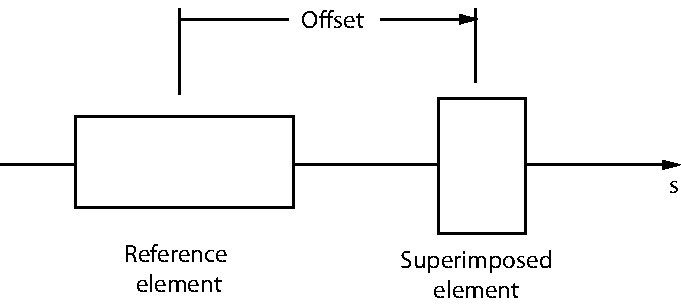
\includegraphics{superimpose.pdf} 
\caption[Superposition Illustration.]
{Illustration of a superposition.}
\label{f:superimpose}
\end{figure}

With the lattice broken up like this \bmad has constructed something
that can be easily analyzed. However, the original elements \vn{Q} and
\vn{S} still exist within the lord section of the lattice. \bmad has
bookkeeping routines so that if a change is made to the \vn{Q} or
\vn{S} elements then these changes can get propagated to the
corresponding slaves. It does not matter which element is
superimposed. Thus, in the above example, \vn{S} could have been put
in the Beam Line (with a drift before it) and \vn{Q} could then have
been superimposed on top and the result would have been the same
(except that the split elements could have different names).

If a zero length element, such as a marker, is superimposed with some
other element (or vice versa) the element is just split in two. For
example:
\begin{example}
  Q: quad, l = 10
  M: marker, superimpose, offset = 6
  lat: line = (Q)
  use, lat
\end{example}
The resulting is that the tracking part of the lattice would be
\begin{example}
        Element   Key           Length
  1)    Q{\#}1       Quadrupole    6
  2)    M         Marker        0
  3)    Q{\#}2       Quadrupole    4
\end{example}
and the lord part of the lattice would have the \vn{Q} element.
 
A superposition is illustrated in \fig{f:superimpose} The
placement of a superimposed element is determined by three factors: A
reference point on the superimposed element, a reference point in the
lattice line, and an offset between the points. The attributes that
determine these three quantities are: 
\index{ref}\index{offset}
\index{ref_beginning}\index{ref_center}\index{ref_end}
\index{ele_beginning}\index{ele_center}\index{ele_end}
\begin{example}
  ref = <element name in lattice>
  offset = <length>      (default = 0)
  ref_beginning
  ref_center             (default)
  ref_end
  ele_beginning
  ele_center             (default)
  ele_end
\end{example}
\vn{ref} sets the reference element. If \vn{ref} is not present then
the start of the lattice is used. \vn{ref_beginning}, \vn{ref_center}
or \vn{ref_end} can be used to indicate where on the reference element
the reference point is. Default is \vn{ref_center}. Similarly,
\vn{ele_beginning}, \vn{ele_center}, or \vn{ele_end} can be used to
indicate the reference point on the superimposed element at the
beginning (entrance) edge, the center, or the end (exit) edge
respectively. If neither of these attributes are given the default is
to use the element center. \vn{offset} is the longitudinal offset
between the reference point on the reference element and the reference
point on the superimposed element. The default if not present is zero.

\index{geometry}
\index{open}
\index{drift}
\index{overlay}
\index{group}
\index{girder}
Superposition may be done with any element except \vn{Drift},
\vn{Group}, \vn{Overlay}, and \vn{Girder} control elements. A
superimposed element that extends beyond either end of the lattice
will be wrapped around so part of the element will be at the beginning
of the lattice and part of the element will be at the end. For
consistency's sake, this is done even if the \vn{geometry} is set
to \vn{open} (for example, it is sometimes convenient to
treat a circular lattice as linear). Example:
\begin{example}
  d: drift, l = 10
  q: quad, l = 2, superimpose
  machine: line = (d)
  use, machine
\end{example}
The lattice will have three elements in the tracking section:
\begin{example}
        Element   Key           Length
  3)    Q{\#}2       Quadrupole    1
  2)    D{\#}1       Drift         8
  1)    Q{\#}1       Quadrupole    1
\end{example}
The lord section of the lattice will have the element \vn{Q}. 

\index{drift!superposition}\index{pipe!superposition}
When a superposition is made that overlaps a drift the drift, not
being a "real" element, vanishes. That is, it does not get put in the
lord section of the lattice.  Note that if aperture limits
(\sref{s:limit}) have been assigned to a drift, the aperture limits
can ``disappear'' when the superposition is done. Explicitly, if the
exit end of a drift has been assigned aperture limits, the limits will
disappear if the superimposed element overlays the exit end of the
drift. A similar situation applies to the entrance end of a drift. If
this is not desired, use a \vn{pipe} element instead.

%-----------------------------------------------------------------------------
\subsection{Changing Element Lengths when there is Superposition}
\label{s:super.length}

\index{overlay}
\index{group}
\index{expand_lattice}
When the lattice is constructed, superposition of elements is done
before the addition of any \vn{group} or \vn{overlay} elements. This
is done since \vn{overlay}s and \vn{group}s are allowed to refer
to elements that are superimposed. This can lead to some unexpected
results. For example:
\begin{example}
  q1: quad, l = 10
  q2: quad, l = 10
  lat: line = (q1, q2)
  use, lat
  o: overlay = {q1}, l = 12
  m: marker, superimpose, offset = 15
\end{example} 
In this example, the marker is initially positioned at 15~meters from
the beginning of the lattice.  The application of the overlay will
increase the length of \vn{q1} by 2~meters which will push the marker
\vn{m} to 17~meters which might not be what was intended. To avoid
this problem, an \vn{expand_lattice} statement (\sref{s:expand}) can
be placed after the overlay, but before the superimpose, statement
\begin{example}
  ...
  o: overlay = {q1}, l = 12
  expand_lattice
  m: marker, superimpose, offset = 15
\end{example} 

The length of a superimposed element must necessarily be equal to the
sum of the lengths of its slave elements. For example, the element
\vn{S} in the first example of Section~\sref{s:super} has a length of
6~meters which is equal to the sum of the length of \vn{Q{\B}S}
(3~meters) plus the length of \vn{S{\#1}} (also 3~meters).

If the length of a superimposed element is varied after the lattice
has been expanded, the length of the slaves will be adjusted
accordingly. For example, if, after lattice expansion, the length of
element \vn{S} in the first example of Section~\sref{s:super} is
increased by 50\% from 6~meters to 9~meters, the lattice would look
like
\begin{example}
        Element   Key         Length  Total
  1)    Q{\#}1       Quadrupole   4        4
  2)    Q{\B}S       Sol_quad     6       10
  3)    S{\#}1       Solenoid     3       13
  4)    D{\#}2       Drift        8       21
\end{example}
The length of \vn{Q{\B}S} has been increased by 50\% from 4~meters to
6~meters and the length of \vn{S{\#}1} has been increased by 50\% from
2~meters to 3~meters to give the proper length for \vn{S}.
Additionally, to keep the length of \vn{Q} at 10~meters, the
length of \vn{Q{\#}1} has been decreased to 4~meters. The overall
length of the lattice has increased by 1~meter.

Notice that this result is {\em not} what would be obtained if the
length of the element \vn{S} is increased to 9~meters in the lattice
file. The reason for this incompatibility stems from the fact that the
effect of varying an element's length in the lattice file depends upon
what reference points are used for specifying any superpositions. For
example, if the reference point of \vn{S} in the first example of
Section~\sref{s:super} is changed to
\begin{example}
  S: solenoid, l = 6, superimpose, ele_beginning, offset = 6
\end{example}
The expanded lattice is unaltered. But with this shifted reference
point, the effect of changing the length of \vn{S} is different. That is
\begin{example}
  S: solenoid, l = 7, superimpose, ref = q, ref_end, offset = -1
\end{example}
will not produce the same expanded lattice as
\begin{example}
  S: solenoid, l = 7, superimpose, ele_beginning, offset = 6
\end{example}
Thus if someone using a simulation program is only considering the
expanded lattice, there is the potential for confusion if length
changes mirrored the effect of changing the lengths in the lattice
file.  To avoid this, and to simplify the computational overhead,
\bmad chooses to use a relatively simple algorithm for adjusting
lengths after lattice expansion. Notice that for layout design, the
\vn{no_superimpose} command (\sref{s:debug}) can be used to
suppress superposition.
